%% For normal draft builds (figs undisplayed hence fast compile)
%\documentclass[hyperpdf,nobind,draft,oneside]{hepthesis}
%\documentclass[hyperpdf,nobind,draft,twoside]{hepthesis}

%% For short draft builds (breaks citations by necessity)
%\documentclass[hyperpdf,nobind,draft,hidefrontback]{hepthesis}

%%For Cambridge soft-bound version
\documentclass[hyperpdf,bindnopdf]{hepthesis}
%% For Cambridge hard-bound version (must be one-sided)
%\documentclass[hyperpdf,oneside]{hepthesis}

%% Load special font packages here if you wish
%\usepackage{lmodern}

\usepackage{mathpazo}
\usepackage{xeCJK}

\usepackage{titlesec}
\usepackage{multirow}
\usepackage{indentfirst}
\usepackage{longtable, booktabs}

\titleformat{\chapter}
  {\normalfont\huge\bfseries}{第\thechapter 章.}{20pt}{\huge}

%\usepackage{euler}

\renewcommand\tablename{表}
\renewcommand*\contentsname{目录}

%% Put package includes etc. into preamble.tex for convenience
\usepackage{xspace}
\usepackage{tikz}
\usepackage{morefloats,subfig,afterpage}
\usepackage{mathrsfs} % script font
\usepackage{verbatim}

%% Using Babel allows other languages to be used and mixed-in easily
%\usepackage[ngerman,english]{babel}
\usepackage[english]{babel}
\selectlanguage{english}

%% Citation system tweaks
\usepackage{cite}
% \let\@OldCite\cite
% \renewcommand{\cite}[1]{\mbox{\!\!\!\@OldCite{#1}}}

%% Maths
% TODO: rework or eliminate maybemath
\usepackage{abmath}
\DeclareRobustCommand{\mymath}[1]{\ensuremath{\maybebmsf{#1}}}
% \DeclareRobustCommand{\parenths}[1]{\mymath{\left({#1}\right)}\xspace}
% \DeclareRobustCommand{\braces}[1]{\mymath{\left\{{#1}\right\}}\xspace}
% \DeclareRobustCommand{\angles}[1]{\mymath{\left\langle{#1}\right\rangle}\xspace}
% \DeclareRobustCommand{\sqbracs}[1]{\mymath{\left[{#1}\right]}\xspace}
% \DeclareRobustCommand{\mods}[1]{\mymath{\left\lvert{#1}\right\rvert}\xspace}
% \DeclareRobustCommand{\modsq}[1]{\mymath{\mods{#1}^2}\xspace}
% \DeclareRobustCommand{\dblmods}[1]{\mymath{\left\lVert{#1}\right\rVert}\xspace}
% \DeclareRobustCommand{\expOf}[1]{\mymath{\exp{\!\parenths{#1}}}\xspace}
% \DeclareRobustCommand{\eexp}[1]{\mymath{e^{#1}}\xspace}
% \DeclareRobustCommand{\plusquad}{\mymath{\oplus}\xspace}
% \DeclareRobustCommand{\logOf}[1]{\mymath{\log\!\parenths{#1}}\xspace}
% \DeclareRobustCommand{\lnOf}[1]{\mymath{\ln\!\parenths{#1}}\xspace}
% \DeclareRobustCommand{\ofOrder}[1]{\mymath{\mathcal{O}\parenths{#1}}\xspace}
% \DeclareRobustCommand{\SOgroup}[1]{\mymath{\mathup{SO}\parenths{#1}}\xspace}
% \DeclareRobustCommand{\SUgroup}[1]{\mymath{\mathup{SU}\parenths{#1}}\xspace}
% \DeclareRobustCommand{\Ugroup}[1]{\mymath{\mathup{U}\parenths{#1}}\xspace}
% \DeclareRobustCommand{\I}[1]{\mymath{\mathrm{i}}\xspace}
% \DeclareRobustCommand{\colvector}[1]{\mymath{\begin{pmatrix}#1\end{pmatrix}}\xspace}
\DeclareRobustCommand{\Rate}{\mymath{\Gamma}\xspace}
\DeclareRobustCommand{\RateOf}[1]{\mymath{\Gamma}\parenths{#1}\xspace}

%% High-energy physics stuff
\usepackage{abhep}
\usepackage{hepnames}
\usepackage{hepunits}
\DeclareRobustCommand{\arXivCode}[1]{arXiv:#1}
\DeclareRobustCommand{\CP}{\ensuremath{\mathcal{CP}}\xspace}
\DeclareRobustCommand{\CPviolation}{\CP-violation\xspace}
\DeclareRobustCommand{\CPv}{\CPviolation}
\DeclareRobustCommand{\LHCb}{LHCb\xspace}
\DeclareRobustCommand{\LHC}{LHC\xspace}
\DeclareRobustCommand{\LEP}{LEP\xspace}
\DeclareRobustCommand{\CERN}{CERN\xspace}
\DeclareRobustCommand{\bphysics}{\Pbottom-physics\xspace}
\DeclareRobustCommand{\bhadron}{\Pbottom-hadron\xspace}
\DeclareRobustCommand{\Bmeson}{\PB-meson\xspace}
\DeclareRobustCommand{\bbaryon}{\Pbottom-baryon\xspace}
\DeclareRobustCommand{\Bdecay}{\PB-decay\xspace}
\DeclareRobustCommand{\bdecay}{\Pbottom-decay\xspace}
\DeclareRobustCommand{\BToKPi}{\HepProcess{ \PB \to \PK \Ppi }\xspace}
\DeclareRobustCommand{\BToPiPi}{\HepProcess{ \PB \to \Ppi \Ppi }\xspace}
\DeclareRobustCommand{\BToKK}{\HepProcess{ \PB \to \PK \PK }\xspace}
\DeclareRobustCommand{\BToRhoPi}{\HepProcess{ \PB \to \Prho \Ppi }\xspace}
\DeclareRobustCommand{\BToRhoRho}{\HepProcess{ \PB \to \Prho \Prho }\xspace}
\DeclareRobustCommand{\X}{\thesismath{X}\xspace}
\DeclareRobustCommand{\Xbar}{\thesismath{\overline{X}}\xspace}
\DeclareRobustCommand{\Xzero}{\HepGenParticle{X}{}{0}\xspace}
\DeclareRobustCommand{\Xzerobar}{\HepGenAntiParticle{X}{}{0}\xspace}
\DeclareRobustCommand{\epluseminus}{\Ppositron\!\Pelectron\xspace}
\DeclareRobustCommand{\protonproton}{\Pproton\APantiproton\xspace}


%% You can set the line spacing this way
%\setallspacing{double}
%% or a section at a time like this
%\setfrontmatterspacing{double}

%% Define the thesis title and author
\title{网络技术挑战赛\\4over6原理验证系统\\开发文档}
\author{ }

%% Doc-specific PDF metadata
\makeatletter
\@ifpackageloaded{hyperref}{%
\hypersetup{%
  pdftitle = {Studying B to K pi decays with LHCb},
  pdfsubject = {Andy Buckley's PhD thesis},
  pdfkeywords = {LHCb, B, physics, LHC, heavy flavour},
  pdfauthor = {\textcopyright\ Andy Buckley}
}}{}
\makeatother


%% Start the document
\begin{document}

%% Define the un-numbered front matter (cover pages, rubrik and table of contents)
\begin{frontmatter}
  %% Title
\titlepage[\quad]{\quad}

%% Abstract
%\begin{abstract}%[\smaller \thetitle\\ \vspace*{1cm} \smaller {\theauthor}]
%  %\thispagestyle{empty}
%  \LHCb is a \bphysics detector experiment which will take data at
%  the \unit{14}{\TeV} \LHC accelerator at \CERN from 2007 onward\dots
%\end{abstract}


%% Declaration
%\begin{declaration}
%  This dissertation is the result of my own work, except where explicit
%  reference is made to the work of others, and has not been submitted
%  for another qualification to this or any other university. This
%  dissertation does not exceed the word limit for the respective Degree
%  Committee.
%  \vspace*{1cm}
%  \begin{flushright}
%    Andy Buckley
%  \end{flushright}
%\end{declaration}


%% Acknowledgements
%\begin{acknowledgements}
%  Of the many people who deserve thanks, some are particularly prominent,
%  such as my supervisor\dots
%\end{acknowledgements}


%% Preface
%\begin{preface}
%  This thesis describes my research on various aspects of the \LHCb
%  particle physics program, centred around the \LHCb detector and \LHC
%  accelerator at \CERN in Geneva.
%
%  \noindent
%  For this example, I'll just mention \ChapterRef{chap:SomeStuff}
%  and \ChapterRef{chap:MoreStuff}.
%\end{preface}

%% ToC
\tableofcontents


%% Strictly optional!
%\frontquote{%
%  Writing in English is the most ingenious torture\\
%  ever devised for sins committed in previous lives.}%
%  {James Joyce}
%% I don't want a page number on the following blank page either.
\thispagestyle{empty}

\end{frontmatter}

%% Start the content body of the thesis
\begin{mainmatter}
  %% Actually, more semantic chapter filenames are better, like "chap-bgtheory.tex"
  \chapter{项目简介}


\section{项目概述}
% 本条应简述本文档适用的系统和软件的用途。它应描述系统与软件的一般性质;概述系统开发、运行和维护的历史;标识项目的投资方、需方、用户、开发方和支持机构;标识当前和计划的运行现场;并列出其他有关文档。

IPV4 over IPV6,简称“4over6”是IPV4向IPV6发展进程中,向纯IPV6主干网过渡提出的一种新技术,可以最大程度地继承基于IPV4网络和应用,实现IPV4向IPV6平滑的过渡。
该项目通过实现IPV4 over IPV6隧道最小原型验证系统,以实现在安卓手机上,通过IPv6网络访问IPv4网站的功能。 


% \section{项目目的}
% % 本条应包含本文档适用的系统和软件的完整标识,(若适用)包括标识号、标题、缩略词语、版本号、发行号。

% \begin{itemize}
%     \item 掌握Android下应用程序开发环境的搭建和使用
%     \item 掌握IPv4 over IPv6隧道的工作原理
% \end{itemize}

\section{客户端项目概述}
% 本条应概括本文档的用途与内容,并描述与其使用有关的保密性与私密性要求。
在安卓设备上实现一个4over6隧道系统的客户端程序,内容如下:

\begin{itemize}
    \item 实现安卓界面程序,显示隧道报文收发状态(java语言)
    \item 启用安卓VPN服务(java语言)
    \item 实现底层通信程序,对4over6隧道系统控制消息和数据消息的处理(C语言)
\end{itemize}

\section{服务器项目概述}

在linux系统下,实现4over6隧道系统服务端程序,内容如下:
\begin{itemize}
    \item 实现服务端与客户端之间控制通道的建立与维护
    \item 实现对客户端网络接口的配置
    \item 实现对4over6隧道系统数据报文的封装和解封装
\end{itemize}
  \chapter{项目原理}
\label{chap:SomeStuff}

\pagenumbering{arabic}

\section{面向Android终端的隧道原理}

IPv6网络中的用户在希望访问IPv4服务时,将IPv4包封装在IPv6包中发送给一台能够直接访问IPv4服务的服务器。
该服务器将进行实际IPv4资源的访问,然后再将得到的IPv4响应封装在IPv6包中发送回用户。
为了能够通过IPv4地址将IPv4响应返回给相应的用户,IPv4 over IPv6服务器需要维护一个IPv4和IPv6地址的映射表并为需要IPv4 over IPv6服务的用户分配IPv4地址。
本次项目中的IPV4 over IPV6隧道原理如下图所示:
\begin{figure}[!ht]
	\begin{center}
	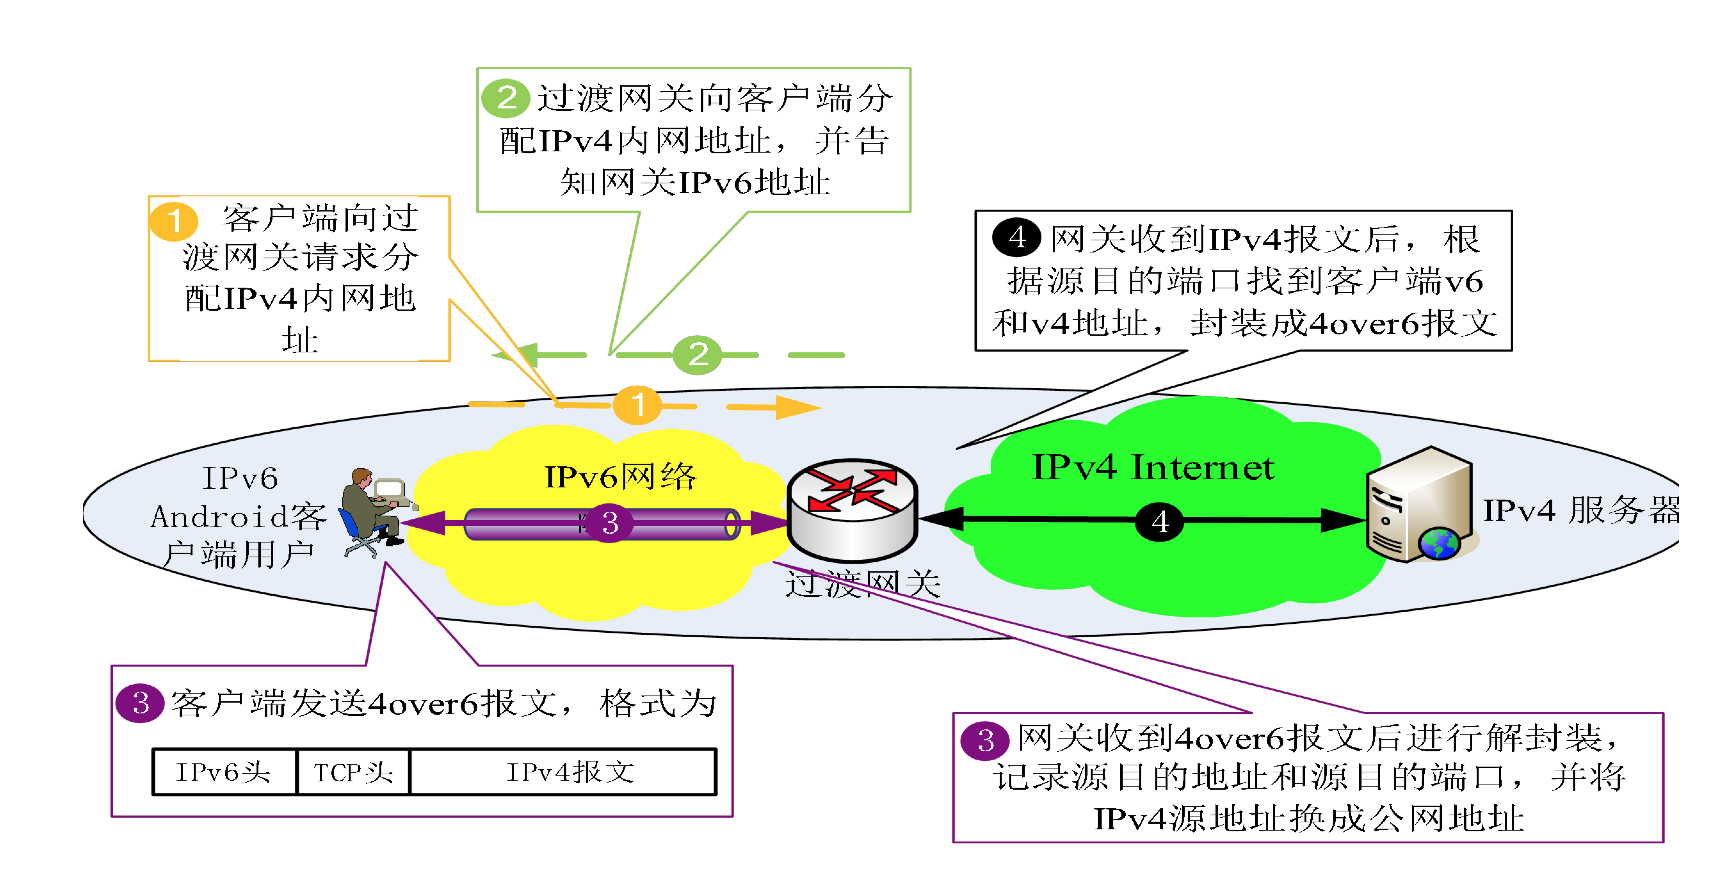
\includegraphics[scale=.58]{4over6.png}
	\end{center}
	\caption{面向Android终端的隧道原理}
	\label{figure:4over6}
\end{figure}
\\ 在本次项目中,我们用到的隧道原理主要是面向Android终端的隧道原理,在面向Android终端的隧道原理中,大致流程为:
安卓客户端首先向过渡网关请求分配 IPv4 内网地址;过渡网关向客户端分配 IPv4 内网地址,并提供对应的 IPv6 网络地址;
接着,安卓客户端发送 IPv4 over IPv6 报文;网关收到报文后解封装,记录源目的地址和源目的端口,并将 IPv4 源地址换成公网地址。
当过渡网关收到来自 IPv4 服务器的报文之后,会根据之前 记录的映射关系,重新封装成 IPv4 over IPv6 报文,发送给对应的内网用户,这样就完成了数据的的转发和接收,用户便可以成 功接收到 IPv4 数据,从而实现通过IPv6网络访问IPv4的功能。


\section{项目网络拓扑}

本次项目中用到的网络拓扑如下图所示:
\begin{figure}[!ht]
\begin{center}
	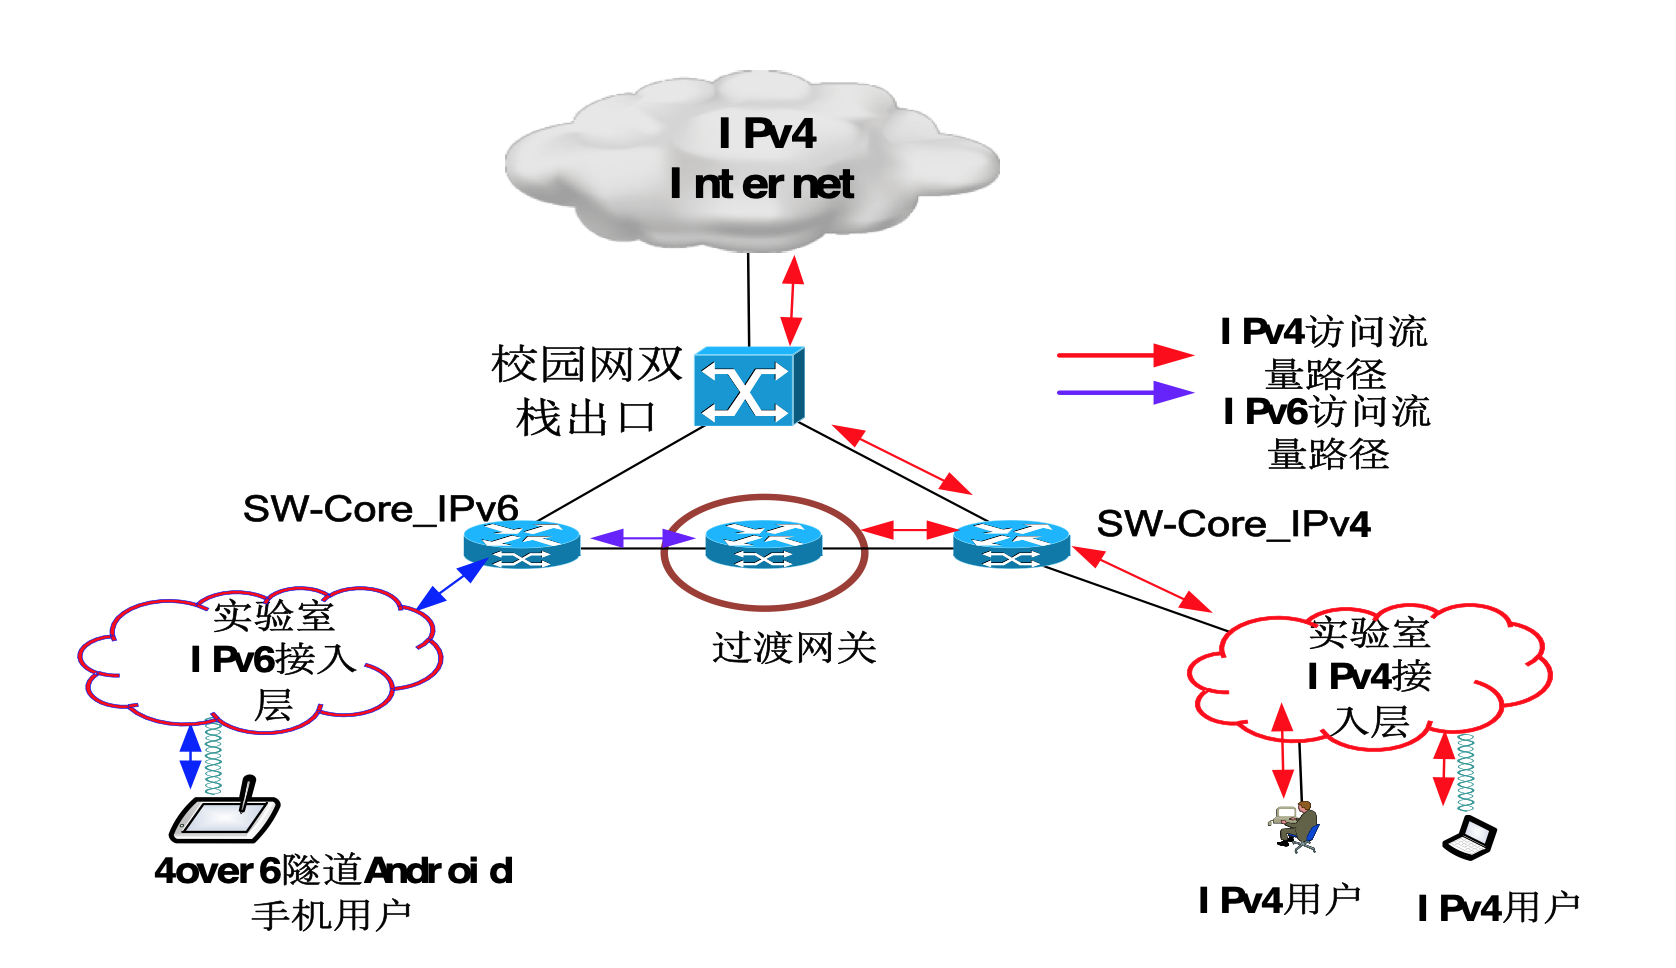
\includegraphics[scale=.58]{network.png}
    \end{center}
    \caption{项目网络拓扑图}
    \label{figure:network}
\end{figure}

\section{安卓VPN Service原理}

VPN Service是一个android自带的vpn服务类,它可以在你不root手机的情况下,实现对你手机流量控制。可以通过设置对指定应用流量的拦截,也可以做全局操作。
如果你的应用是想要拦截网络,或者想要,获取网络数据,转发网络数据,就可以通过这个去做。VPN Service 会监控所有的网络进程,并可以进行 IP 隧道处理。
当我们发送数据时,可以使用 IPv6 包装要发送的报文并发送给网关。
当我们接收数据时,可 以将 IPv4 的报文从数据包中剥离出来。
本次项目中,安卓客户端需要完成 IPv4 over IPv6 报文的封装和解封装,我们采用了 VPN Service 来进行实现。
VPN Service 是安卓的一套 API 接口,方便编程人员创 建 VPN 服务。
打开服务之后,安卓系统将所有的应用程序发送的 IP 包都根据 iptables 使用 NAT 转发到 TUN,其端口为 tun0。
当打开 VPN Service 之后,我们可 以获取 tun0 的文件描述符,这样就可以读取或写入数据以实现发送或者接收数据。

Android设备上,已经使用了VpnService框架,建立起了一条从设备到远端的VPN链接
\begin{itemize}
\item 应用程序使用socket,将相应的数据包发送到真实的网络设备上
\item Android系统通过iptables,使用NAT,将所有的数据包转发到TUN虚拟网络设备上去,端口是tun0
\item VPN程序通过打开/dev/tun设备,并读取该设备上的数据,可以获得所有转发到TUN虚拟网络设备上的IP包
\item VPN数据可以做一些处理,然后将处理过后的数据包,通过真实的网络设备发送出去
\end{itemize}

\section{NDK 和 JNI}
在本次项目中,由于经常要和以字节为单位的数据打交道,并且需要精细地管理 内存,因此我们采用 C 来实现 IPv4 over IPv6 的核心功能。
要在以 Java 为语言的安卓 环境中使用 C 来进行编程,因此我们需要使用 JNI 和 NDK。

NDK 是Native Develop Kit的含义,从含义很容易理解,本地开发。大家都知道,Android 开发语言是Java,不过我们也知道,Android是基于Linux的,其核心库很多都是C/C++的,比如Webkit等。那么NDK的作用,就是Google为了提供给开发者一个在Java中调用C/C++代码的一个工作。NDK本身其实就是一个交叉工作链,包含了Android上的一些库文件,然后,NDK为了方便使用,提供了一些脚本,使得更容易的编译C/C++代码。总之,在Android的SDK之外,有一个工具就是NDK,用于进行C/C++的开发。一般情况,是用NDK工具把C/C++编译为.co文件,然后在Java中调用。

JNI,全称为Java Native Interface,即Java本地接口,JNI是Java调用Native 语言的一种特性。通过JNI可以使得Java与C/C++机型交互。即可以在Java代码中调用C/C++等语言的代码或者在C/C++代码中调用Java代码。由于JNI是JVM规范的一部分,因此可以将我们写的JNI的程序在任何实现了JNI规范的Java虚拟机中运行。同时,这个特性使我们可以复用以前用C/C++写的大量代码JNI是一种在Java虚拟机机制下的执行代码的标准机制。代码被编写成汇编程序或者C/C++程序,并组装为动态库。也就允许非静态绑定用法。这提供了一个在Java平台上调用C/C++的一种途径,反之亦然。

  \chapter{项目内容}

\section{客户端}

\subsubsection{客户端前台}
前台是java语言的显示界面
\begin{itemize}
    \item 进行网络检测并获取上联物理接口IPV6地址
    \item 启动后台线程
    \item 开启定时器刷新界面
    \item 界面显示网络状态
    \item 开启安卓VPN服务
\end{itemize}
\subsubsection{客户端后台}
后台是C语言客户端与4over6隧道服务器之间的数据交互
\begin{itemize}
    \item 连接服务器
    \item 获取下联虚接口IPV4地址并通过管道传到前台
    \item VPN程序通过打开/dev/获取前台传送到后台的虚接口描述符
    \item 读写虚接口
    \item 对数据进行解封装
    \item 通过IPV6套接字与4over6隧道服务器进行数据交互
    \item 实现保活机制,定时给服务器发送keeplive消息
\end{itemize}

\section{服务器端}
服务端在linux环境下运行,主要有下面几个功能:
\begin{itemize}
    \item 创建IPV6 TCP套接字,监听服务器和客户端之间的数据通信
    \item 维护虚接口,实现对虚接口的读写操作
    \item 维护IPV4地址池,实现为新连接客户端分配IPV4地址
    \item 维护客户信息表,保存IPV4地址与IPV6套接字之间的映射关系
    \item 读取客户端从IPV6 TCP套接字发送来的数据,实现对系统的控制消息和数据消息的处理
    \item 实现对数据消息的解封装,并写入虚接口
    \item 实现对虚接口接收到的数据报文进行封装,通过IPV6套接字发送给客户端
    \item 实现保活机制,监测客户端是否在线,并且定时给客户端发送keeplive消息
\end{itemize}
  \chapter{项目设计与实现}
在本次项目中,我们的项目主要分为两大部分,客户端和服务器端。

客户端可以分为两大部分,前台和后台,前台是安卓界面的显示,后台是创建IPV6套接字,数据的封装与解封装,以及与4over6隧道服务端的通信。
本次项目中的客户端整体流程如图4.1所示:
\begin{figure}[!ht]
	\begin{center}
	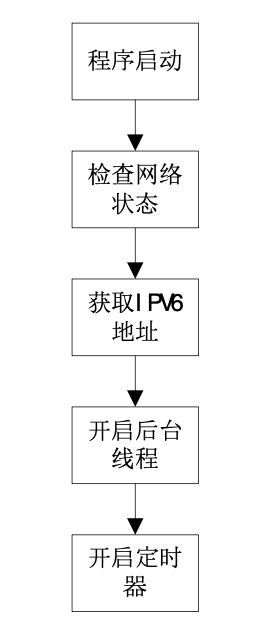
\includegraphics[scale=.58]{client_all.png}
	\end{center}
	\caption{客户端整体流程}
	\label{figure:客户端整体流程图}
\end{figure}

\begin{itemize}
  \item 程序启动后,先检查网络状态
  \item 获取IPV6地址
  \item 开启后台线程
  \item 开启前台定时器刷新界面(间隔1秒)
\end{itemize}

前台是java语言的显示界面,后台是C语言的数据交互,前后台之间通过管道进行通信,这里创建了两个管道,一个是IP信息管道,一个是流量信息管道,两个管道分开处理相对简单,通信的详细流程如图4.2下所示:
\begin{figure}[!ht]
	\begin{center}
	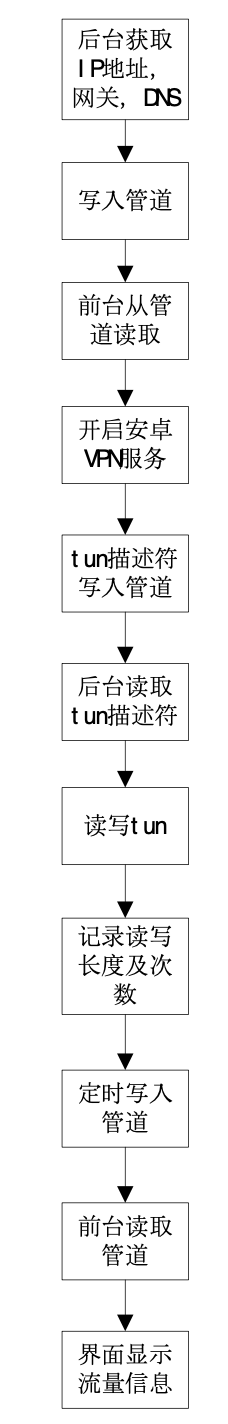
\includegraphics[scale=.58]{front_back.png}
	\end{center}
	\caption{前后台通信流程}
	\label{figure:前后台通信流程图}
\end{figure}

\begin{itemize}
  \item 后台获取到4over6服务器发送来的IP地址等信息
  \item 把这些信息解析出来,写入IP信息管道
  \item 前台从IP信息管道读取到IP地址等信息
  \item 开启安卓VPN服务
  \item 把安卓虚接口描述符写入IP信息管道
  \item 后台从IP信息管道获取安卓虚接口文件描述符
  \item 对该虚接口进行读写操作
  \item 记录读写长度和次数
  \item 在后台定时器线程,定时写入流量信息管道
  \item 前台从流量信息管道获取流量信息
  \item 定时刷新界面的流量信息
\end{itemize}

服务器端主要可以分为三部分:主进程循环、读取虚接口线程、keeplive线程。主框架流程图如图4.3下所示:
\begin{figure}[!ht]
	\begin{center}
	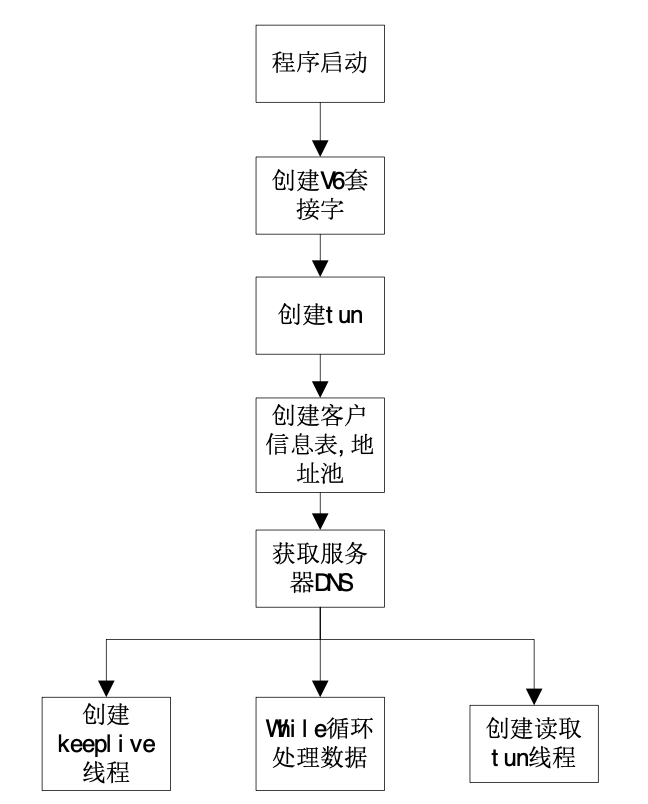
\includegraphics[scale=.58]{server_all.png}
	\end{center}
	\caption{服务器端整体流程}
	\label{figure:服务器端整体流程图}
\end{figure}

\begin{itemize}
  \item 创建IPV6套接字,把该套接字加入Select模型字符集
  \item 创建tun虚接口
  \item 创建客户信息表和地址池
  \item 获取服务器DNS地址
  \item 创建keeplive线程
  \item 创建读取虚接口线程
  \item 主进程中while循环中数据处理
\end{itemize}

\section{客户端前台流程设计}
\begin{figure}[!ht]
	\begin{center}
	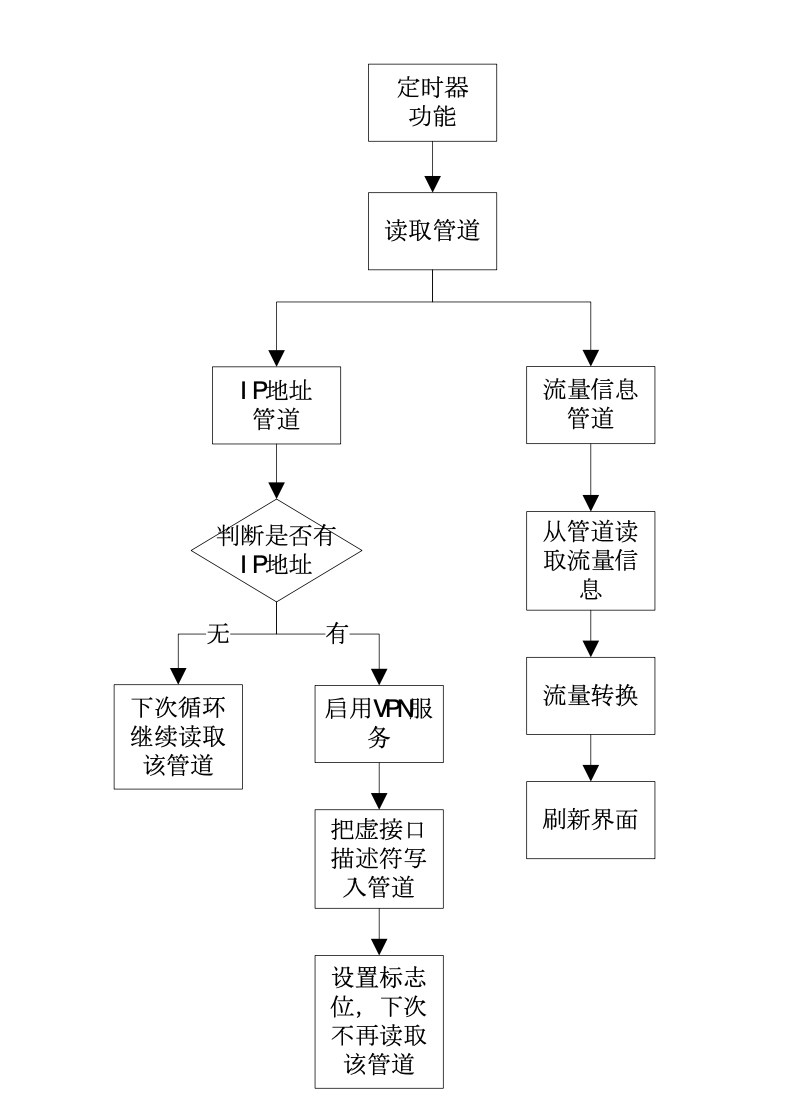
\includegraphics[scale=.58]{front.png}
	\end{center}
	\caption{客户端前台流程设计}
	\label{figure:客户端前台流程设计}
\end{figure}
前台的详细流程图如图4.4所示,前台定时器主要功能为定时刷新显示界面,显示流量信息,定时器功能解析如下:
\begin{itemize}
  \item 开启定时器之前,创建一个读取IP信息管道的全局标志位flag,默认置0
  \item 开始读取管道,首先读取IP信息管道,判断是否有后台传送来的IP等信息。假如没有,下次循环继续读取
  \item 有IP信息,就启用安卓VPN服务
  \item 把获取到的安卓虚接口描述符写入管道传到后台。把flag置1,下次循环不再读取该IP信息管道
  \item 从管道读取后台传来的实时流量信息,把流量信息进行格式转换并显示到界面
  \item 界面显示的信息有运行时长、上传和下载速度、上传总流量和包数、下载总流量和包数、下联虚接口V4地址、上联物理接口IPV6地址
\end{itemize}


\section{客户端前台具体实现}

\subsection{UI主界面}
主界面采用了 ScrollView 嵌套 LinearLayout 的布局方式,将连接 VPN 前后的不同界面通过一个 Layout 展示,通过控制不同组建的可见显示,实现界面的切换。程序界面主要分为 连接VPN前 和 连接VPN后 两个部分。

程序启动时主界面属于连接VPN前界面。其包含两个可输入窗口,分别用于动态设置服务器 IPV6 地址以及服务器端口号。另一个展示栏显示当前本机连接状态以及本机 IPV6 地址。另外两个按钮分别实现连接 VPN 功能以及退出程序功能。当本机网络环境满足需求时,即处于 IPV6 网络环境,可以通过点击【连接 VPN】跳转到连接信息展示界面,此时隐藏初始界面的元素,并将信息展示界面元素显现以实现页面转换。 

连接前程序界面如图4.5所示:
\begin{figure}[!ht]
	\begin{center}
	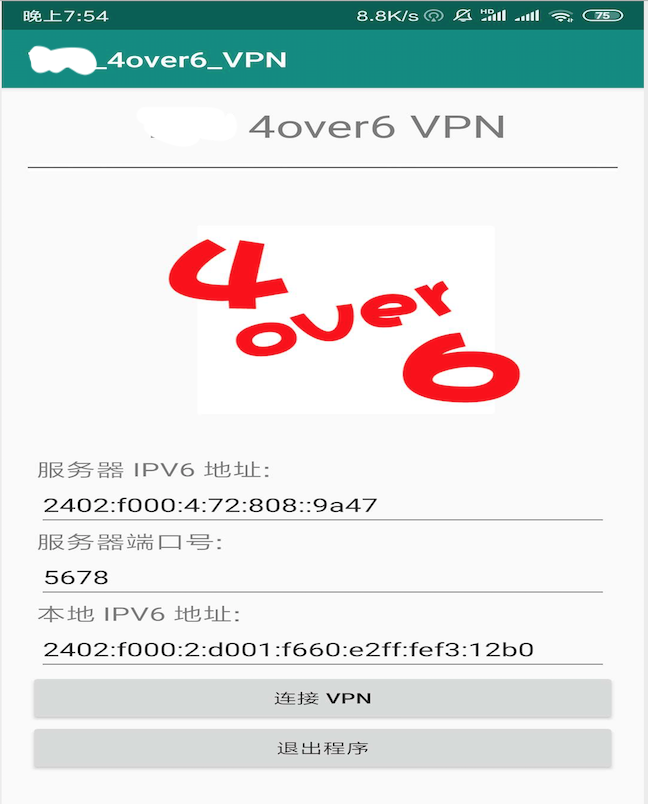
\includegraphics[scale=.58]{connect1.png}
	\end{center}
	\caption{连接前程序界面}
	\label{figure:连接前程序界面}
\end{figure}

连接VPN后 的界面可以展示当前程序运行时间,本机分配的 IPV4 地址,上网速度,总共接收发送包大小等信息。一个【断开 VPN】按钮可以将本机与服务器断开,并回到初始化的界面。

% 连接后程序界面如图4.6所示:
% \begin{figure}[!ht]
% 	\begin{center}
% 	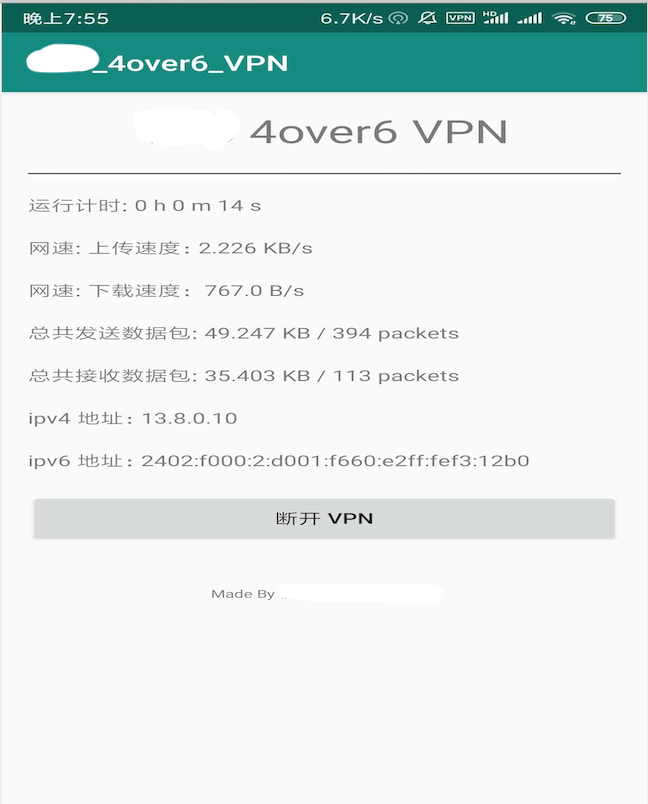
\includegraphics[scale=.58]{connect2.png}
% 	\end{center}
% 	\caption{连接后程序界面}
% 	\label{figure:连接后程序界面}
% \end{figure}

\subsection{MainActivity}
MainActivity 是本程序的主线程,其主要完成程序的初始化工作,以及启动多个线程以支持程序工作。当程序启动时,MainActivity 首先完成对于界面的初始化,为按钮注册监听事件,并每隔 2s 检查本机的网络环境,调用 NetChecker 的 getIpv6Address 尝试获取本机的 IPV6 地址。只有成功获取了本机的 IPV6 地址,才能继续后续的 VPN 服务。

当点击【连接 VPN】按钮后,首先检查是否允许开启 VPN 服务,满足条件会启动 C 后台线程以及前端的定时器线程。C 后台线程见后端具体实现。

前端的定时器线程同前述工作流程。首先连接 IP 信息的管道,接收 C 后台线程传来的 IPV4 地址,DNS 等信息,然后启动 VPN 服务。通过继承 java.util.TimerTask 实现连接 C 后台线程创建的流量信息管道,读取信息并实现 UI 界面信息的更新。 

当点击【断开 VPN】按钮后,会结束 C 后台线程以及前端的定时器线程。

\subsection{MyVpnervice}
MyVpnService 是一个继承了 VpnService 的类,其与主线程 MainActivity 之间通过 Intent 进行数据交换。其需要完成的主要功能是:根据传入的 IPV4 地址,DNS 服务器等参数,初始化 VPN发 服务,并尝试获取虚接口的文件描述符。当获取描述符后,通过管道将数据传给 C 后台。
\subsection{NetChecker}
NetChecker 类主要实现调用 Android 接口,检查本机当前网络环境,并尝试获取 IPV6 地址的功能。isWIFIConnected 负责检查 Wifi 连接状态,getIpv6Address 负责获取本机 IPV6 地址。主线程 MainActivity 只有通过了 NetChecker 类成功获取到本机的 IPV6 地址,才允许前端开启 VPN 服务。 
\section{客户端后台流程设计}
后台流程图如图4.6所示,详细流程解析如下:
\begin{itemize}
  \item 创建IPV6套接字
  \item 连接4over6隧道服务器
  \item 开启定时器线程(间隔1秒)
  \item 发送消息类型为100的IP请求消息
  \item while循环中接收服务器发送来的消息,并对消息类型进行判断
\end{itemize}

\begin{figure}[!ht]
	\begin{center}
	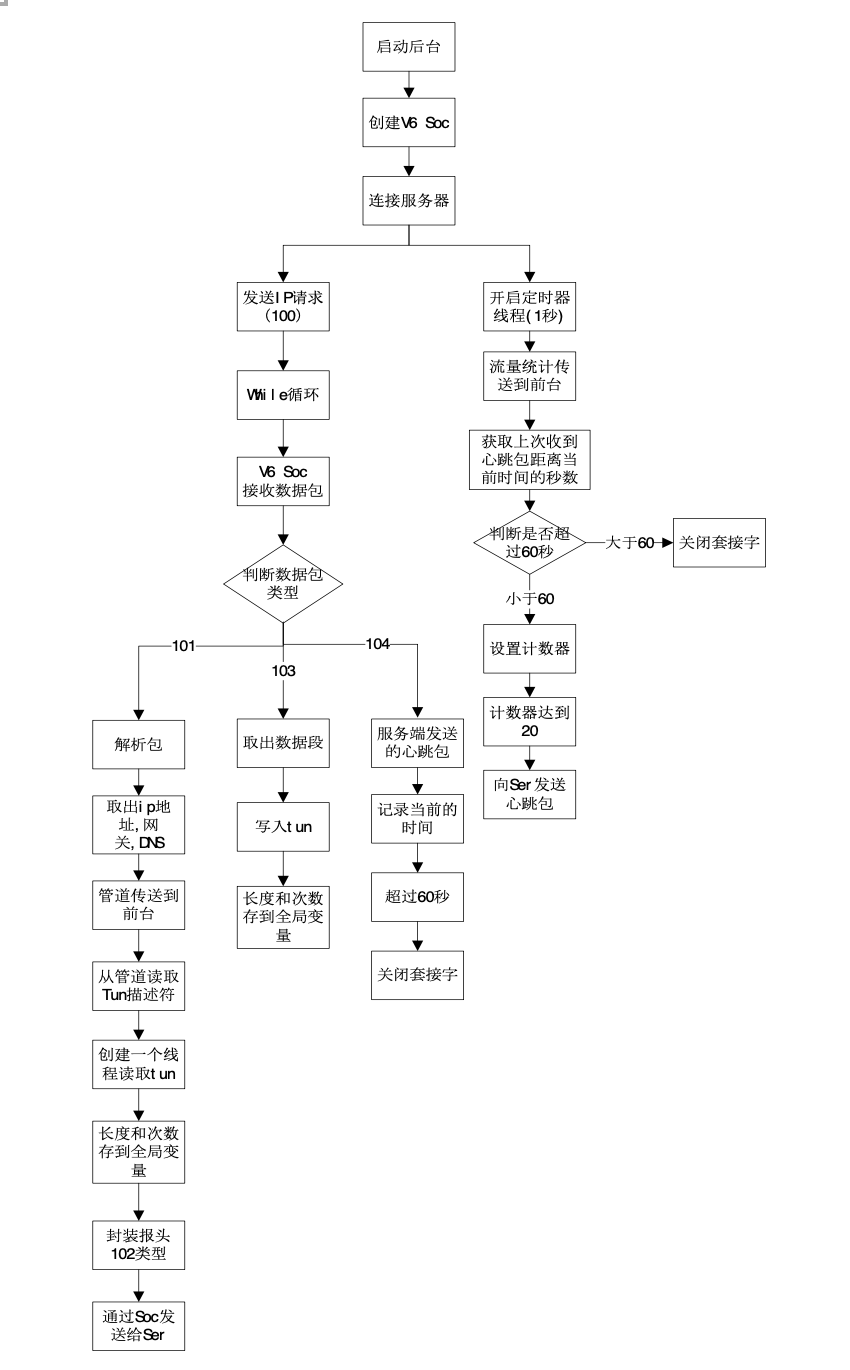
\includegraphics[scale=.58]{back.png}
	\end{center}
	\caption{客户端后台流程设计}
	\label{figure:客户端后台流程设计}
\end{figure}


\section{客户端后台具体实现}
\subsection{JNI}
本次项目需要用 java 代码调用 C 代码,就要用到 JNI。Java Native Interface(JNI) 规定了一套 Java 的原生接口,它提供了若干的 API 实现了 Java 和其他语言的通信(主要是 C和C++)。JNI 是为了本地已编译语言,尤其是 C 和 C++ 而设计的。其支持一个“调用接口”(invocation interface),它允许把一个 JVM 嵌入到本地程序中。本地程序可以链接一个实现了 JVM 的本地库,然后使用“调用接口”执行 JAVA 语言编写的软件模块。
\subsection{后台线程}
当前端启动 C 后台线程时,会传给后台线程服务器的 IPV6 地址以及端口号信息。后端首先进行初始化工作,并建立虚管道,同时使用已有信息创建客户端 Socket,绑定服务器地址,与服务器并进行 TCP 连接。当连接成功时,开启定时器线程 timer\_thread,同时构建 IP 地址请求包,主线程进入 While 循环接收服务器发送来的消息,并对消息类型进行判断,处理数据包。

定时器线程每秒钟会执行一次操作。其主要负责检查与服务器连接是否超时(60s),如果超时则退出 VPN 服务。另外将与服务器连接的相关流量信息(发送/接收包大小,数量)写入管道,并发送至前台,方便前台进行 UI 界面信息的刷新。同时负责每隔 20s 向服务器发送一次心跳包。

主线程在发送 IP 地址请求包后便会进入循环等待并处理服务器发来的数据包。收包的过程是:先构建并清空一个读取缓存 Buffer,首先读取前 4 个字节,代表整个数据包的长度,然后将长度减去 4 之后,按每次一个字节的顺序,逐次读入缓存 Buffer 中,待读取完毕后,将整个 Buffer 拷贝给 Message 即可。根部 Message 的 type 分类,总共需要处理的包有三类(IP地址回应包、上网回应包、心跳包),以下依次讲解:

\begin{itemize}
  \item IP 地址回应包:客户端收到服务器发来的 IP 地址回应包,说明与服务器连接成功。此时需要将数据包中内容(IPV4 地址,DNS 等)经由管道发送给前端,以开启 VPN 服务。完成上述工作后,开启连两个新的线程,一个线程负责循环读取 tun 文件中内容,构造上网请求包发送给服务器;另外一个线程负责持续监听前端是否发来了结束 C 后台线程的指令,以方便结束后台所以运行的线程
  \item 上网回应包:当收到服务器发来的上网回应包时,首先需要统计数据包信息,更新和服务器流量变化,同时需要将数据包内容写入 tun 文件。其中在更新信息时,需要进行加锁操作,实现数据在不同线程间的同步互斥
  \item 心跳包:当收到服务器发来的心跳包,只用更新心跳包收到时间即可,其心跳包发送由定时器线程完成
\end{itemize}

\section{服务器端流程设计}

\subsection{主进程循环}
主进程while循环中主要是Select模型监听所有套接字,然后根据套接字收到数据类型,做不同的处理。while循环如下:
\begin{itemize}
  \item 在while循环中,启用Select模型,对所有的套接字进行监听
  \item 假如监听到服务器套接字,accept新的连接,把新连接的客户端的套接字描述符加入Select字符集
  \item 假如是客户端套接字,首先用ioctl函数判断一下该描述符
  \subitem 假如nread不等于0,客户端正常连接:
    \begin{itemize}
      \item 接收数据
      \item 对收到的数据解封装
      \item 判断数据类型
    \end{itemize}
  \subitem 假如nread等于0,客户端已经断开:
    \begin{itemize}
      \item 遍历客户信息表
      \item 从信息表中查找该客户端描述符所在节点
      \item 取出该节点的IPV4地址
      \item 用该地址与地址池中地址进行匹配
      \item 匹配成功,就把地址池中该地址的标志位置0
      \item 在客户信息表中把该节点删除
      \item Select字符集中清除该描述符
    \end{itemize}
\end{itemize}

while循环流程如图4.7所示:
\begin{figure}[!ht]
	\begin{center}
	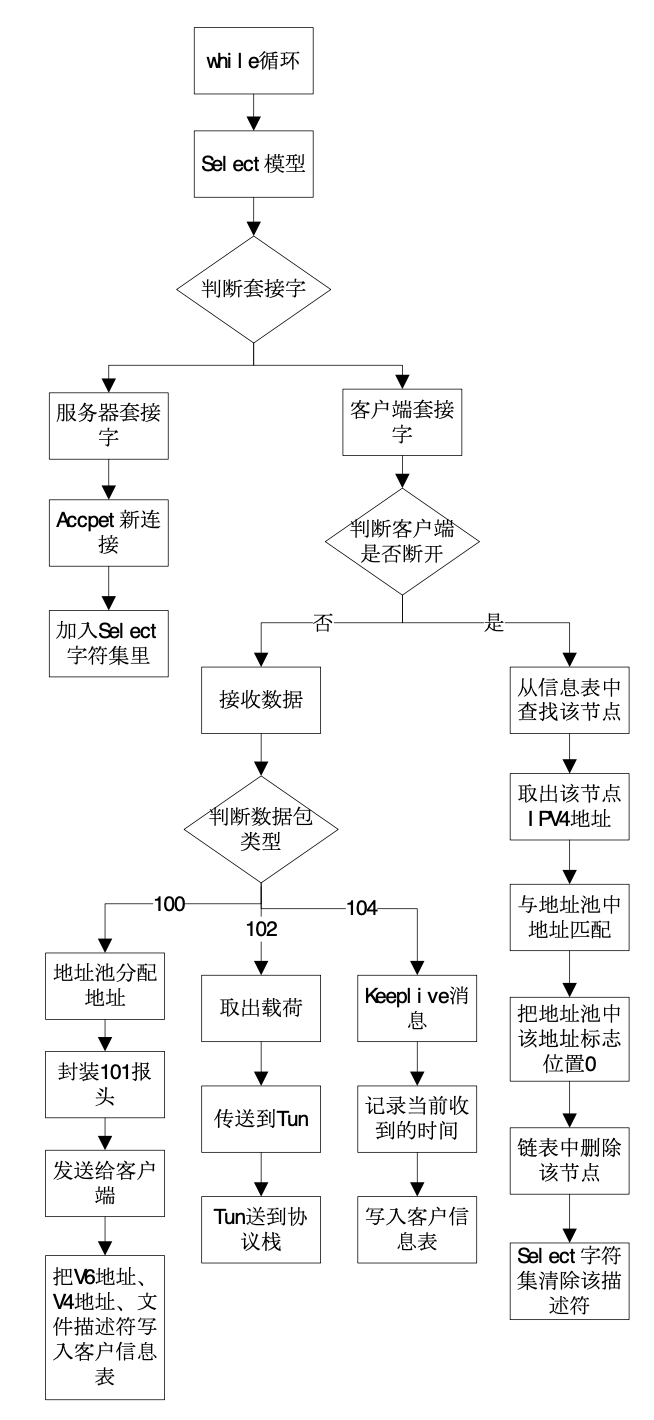
\includegraphics[scale=.58]{server_main.png}
	\end{center}
	\caption{主进程循环流程设计}
	\label{figure:主进程循环流程设计}
\end{figure}

\subsection{读取虚接口线程}

读取虚接口线程主要功能是从协议栈读取消息,根据消息的目的地址,发送给相应的客户端,主要功能如下:
\begin{itemize}
  \item 在while循环中,从虚接口读取消息
  \item 取出该消息的ip头,获取目的ip地址
  \item 遍历客户信息表,查找该目的ip所在的节点
  \item 取出该节点的套接字描述符
  \item 把从虚接口读取到的消息封装103(上网回应)报头
  \item 通过刚才查找到的套接字描述符发送给相应的客户端
\end{itemize}

读取虚接口线程流程如图4.8所示:
\begin{figure}[!ht]
	\begin{center}
	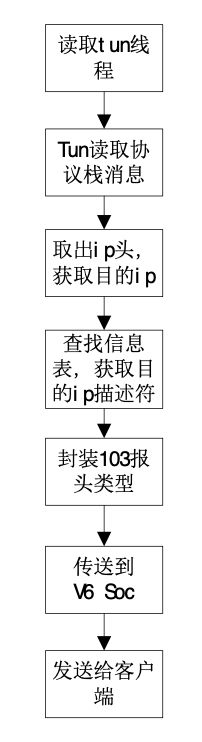
\includegraphics[scale=.58]{server_virtual.png}
	\end{center}
	\caption{读取虚接口线程流程设计}
	\label{figure:读取虚接口线程流程设计}
\end{figure}

\subsection{keeplive线程}
keeplive线程主要功能是给所有当前处于连接状态的客户端发送心跳包,主要功能如下:
\begin{itemize}
  \item sleep一秒钟
  \item 遍历客户信息表
  \item 链表中的每个节点的count字段减1
  \item 当该节点的count字段等于0时,获取该节点的套接字描述符
  \item 通过套接字描述符向该节点所在客户端发送104(心跳包)类型消息
  \item 发送完成,重新把该节点的count字段赋值为20(每隔20秒发送一次心跳包)
  \item 判断每个节点的secs字段的值是否大于60
  \item 假如secs大于60,则说明该客户端已经超过60秒没有给服务器发送心跳包,获取该节点的IPV4地址
  \item 遍历地址池,找到该地址在地址池中所在位置,把该地址的状态字段置为0,回收该地址
  \item 从Select字符集中把该节点的套接字描述符清除,关闭该套接字描述符,删除该节点
\end{itemize}

keeplive线程流程如图4.9所示:
\begin{figure}[!ht]
	\begin{center}
	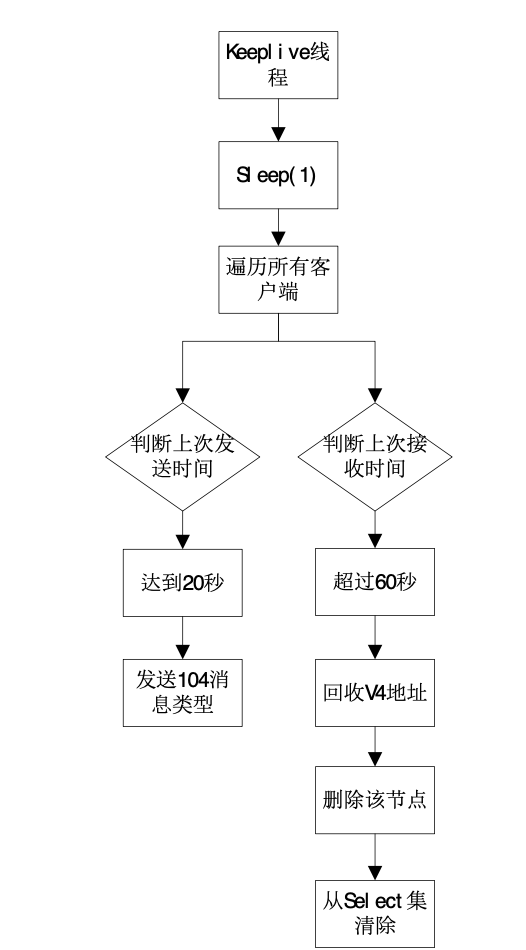
\includegraphics[scale=.58]{server_keep.png}
	\end{center}
	\caption{keeplive线程流程设计}
	\label{figure:keeplive线程流程设计}
\end{figure}

\section{服务器端具体实现}
服务器端大致思路在上述流程设计中已经叙述的足够清楚,在此不再赘述。本部分仅对关键技术要点(NAT、epoll和socket)进行叙述和讲解。
\subsection{NAT}
服务器端使用iptables做NAT,以此实现私有网段和公网地址之间的转换。
当一个客户端发起网络请求时,服务器端的iptables会进行"(客户端IP地址, 端口)即(Src IP, Src Port) -> (服务器端IP地址,端口)即(Dst IP, Dst Port)"之间的映射。 
当公网设备收到上述报文时,服务器端的iptables会根据端口号找到对应客户端的IP地址和监听端口,对该报文的目的地址和目的端口进行替换,这其实是一个逆映射过程。
这样,我们就完成了客户端到服务器端的NAT,实现了私有网段和公网地址之间的转换。

\subsection{epoll和socket}
和网上许多开源的服务器架构一样,我们的项目中,服务器端一样使用了非常便利好用的epoll函数,使用epoll函数同时监听所有客户端对应的socket。
当epoll函数监听到一个可用有效的socket的时候,我们首先会根据这个socket的描述符找到这个socket对应的客户端,然后执行相应的处理函数。
当epoll函数监听到其中任意一个socket状态为“可写”时,则从该客户端对应的数据队列里取出数据写入此socket,持续调用“write()”系统调用直到其返回“EAGAIN”(表明继续写入会导致阻塞),则停止写入。
若epoll函数监听到其中任意一个socket状态为“可读”时,则持续调用“read()”系统调用直到其返回“EAGAIN”(表明当前缓冲区里所有数据都已被读取)。若读到完整的消息,则去掉头部后直接写入隧道。 
我们的隧道同样是使用epoll函数进行监听,不同的是根据实现,每次对隧道调用“read/write”时都会“读/写”一个完整的IP包。从隧道中读到IP包后,则根据IP包头中的Dst IP找到对应的客户端,将该IP包放入对应客户端的数据队列中,待该用户的 socket 可用后发送。
通过上述实现,我们就完成了客户端与服务器端之间的socket连接与信息传输。
 
  \chapter{项目中遇到的问题}

\section{客户端遇到的问题}
我们客户端的开发在项目过程中发现一个问题,即服务器可能向客户端发送不止一个 IP 地址回应包,并且包内容相同。然而在项目中我们仅仅想对 IP 地址回应包进行唯一的一次处理,因为涉及新线程的开启等工作。故我们对于 IP 地址回应包是否进行处理除了判断其数据包类型外,还需要判断是否以前收到了 IP 地址回应包,如果收到了,则将此包丢弃。如果以前没有收到,则处理此包。
\section{服务器端遇到的问题}
服务器端开发我们遇到的最大的问题就是,一开始我们天真的以为客户端和服务器端的开发是完全解耦合的,于是负责客户端开发的同学和负责服务器端开发的同学一开始就是各自为战。但当客户端和服务器端真正一起跑起来之后,才发现并不是像我们想象的那么简单,最大的问题还是服务器端和客户端之间互相通信的问题,服务器能够接收到客户端发来的包,但却无法识别。也就是说服务器端和客户端的包的定义不一致,这也就是说服务器端和客户端并不是完全解耦合的。这一bug的调试极大程度地拖慢了我们的进度,当然最终我们还是成功实现了我们自己开发的服务器端和客户端的通信,并可以成功使用我们的客户端通过我们的服务器进行IPv4 over IPv6的操作。
  \chapter{运行方式及效果}

\section{客户端运行方式}
\begin{itemize}
    \item 开发环境:macOS Mojave 10.14.5
    \item Android Studio版本:3.4
    \item 项目运行手机版本:小米 MIX 2S
\end{itemize}

\section{服务器运行方式}
\begin{itemize}
    \item 开发环境:macOS Mojave 10.14.5
    \item 运行环境:整个服务器项目在具有v4/v6双栈网络的Centos服务器上编译运行
    \item 运行方式:采用Cmake编译运行方式
\end{itemize}

\newpage
\section{最终项目效果}
连接服务器前后界面如图6.1,6.2所示:
\begin{figure}[!ht]
	\begin{center}
	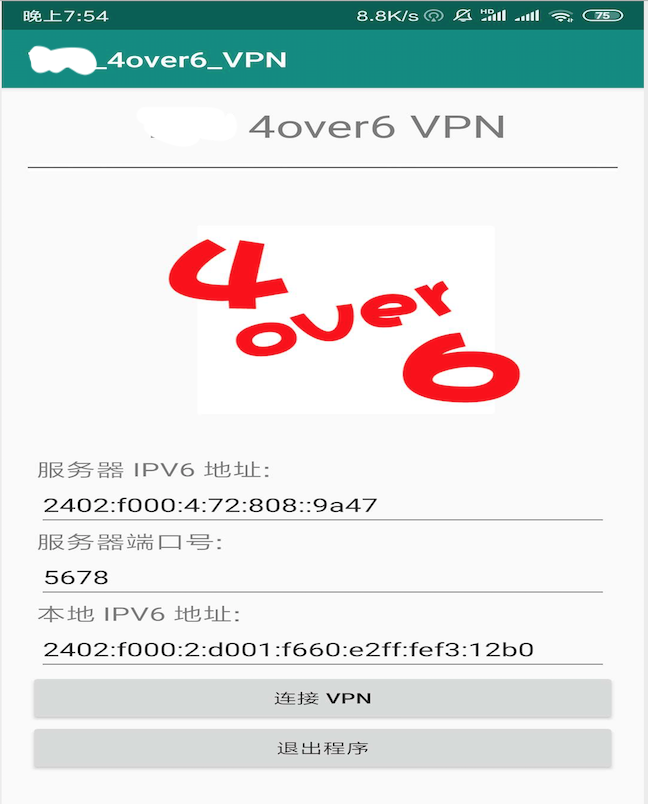
\includegraphics[scale=.58]{connect1.png}
	\end{center}
	\caption{连接服务器前界面}
	\label{figure:连接服务器前界面}
\end{figure}

\begin{figure}[!ht]
	\begin{center}
	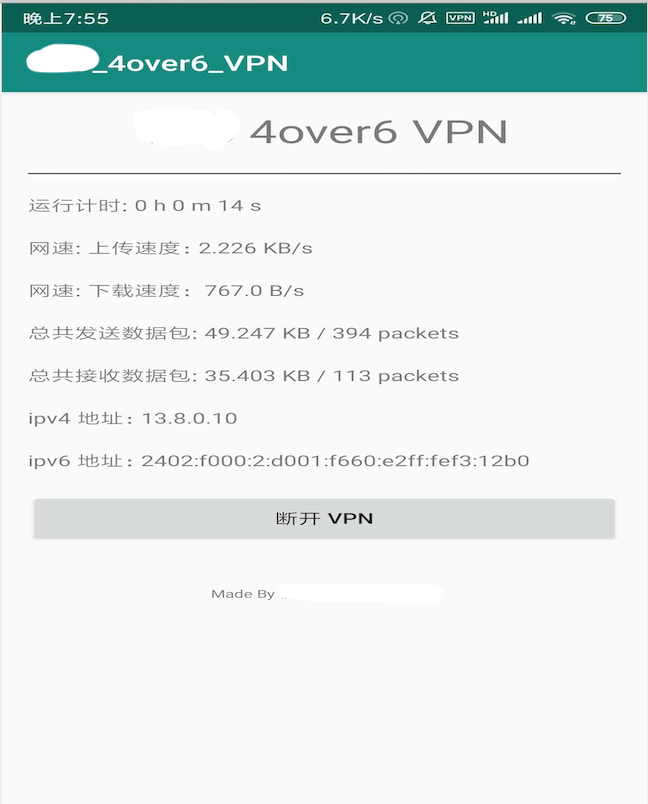
\includegraphics[scale=.58]{connect2.png}
	\end{center}
	\caption{连接服务器后界面}
	\label{figure:连接服务器后界面}
\end{figure}

连接宿舍IPv6网络(未认证账户),使用客户端连接服务器之后访问IPv6网站效果如下:
\begin{figure}[!ht]
	\begin{center}
	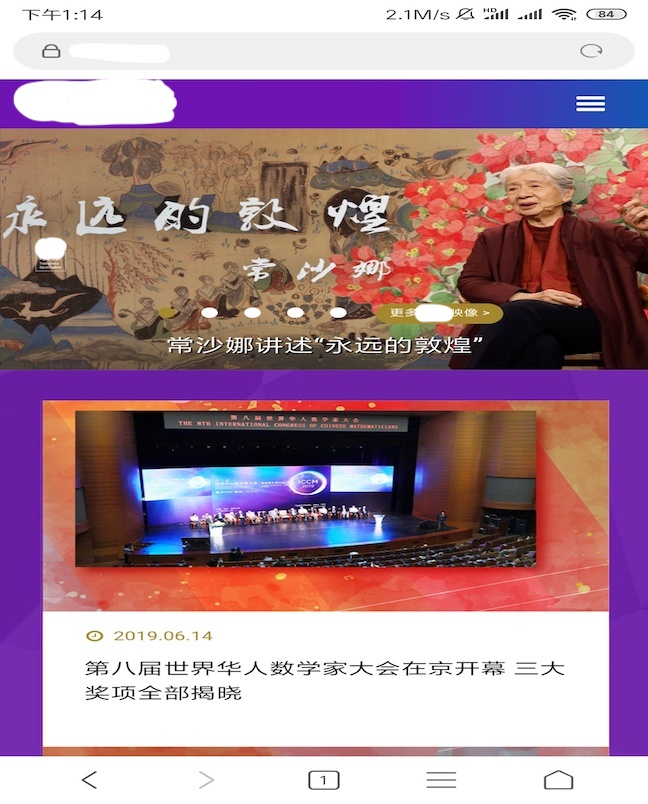
\includegraphics[scale=.58]{tsinghua.jpeg}
	\end{center}
	\caption{访问IPv6网站}
	\label{figure:访问IPv6网站}
\end{figure}

\newpage
连接宿舍IPv6网络(未认证账户),使用客户端连接服务器之后访问IPv4网站效果如下:
\begin{figure}[!ht]
	\begin{center}
	
\includegraphics[scale=.58]{baidu.jpeg}
	\end{center}
	\caption{访问IPv4网站}
	\label{figure:访问IPv4网站}
\end{figure}  
  % \chapter{实验心得与体会}

\section{柳瑞阳同学的心得体会}
在本次课程中,虽然只是有两周的教学讲解,其余时间都大实验时间。但是整体收获依旧很大。需要学习的东西很多。我主要负责4over6客户端的搭建。从一开始的Android Studio环境搭建就费尽不少波折。再到学习Java 内嵌 C 语法,前后台虚拟管道的连接等。虽然这些只是实验的前期准备工作,但是也占用了实验相当大的一部分时间。在这里我要给实验指导书点一个赞,实验指导书内容详尽,为我们提供了不少的帮助。虽然实现流程按照实验指导书编写,但是自己也对于这个流程更加熟悉。助教曾问我:“如果实验指导书不给你们写出来实验实现流程,你们自己能不能实现?”我说,“很玄”。实验指导书为我们实验具体实施提出了明路。但与此同时也有很多坑,在实验指导书中未说明。例如服务器会像客户端多次返回101地址请求包,如果客户端对于每个包都处理,反而会造成不可预见的错误。这个问题的发现也消耗了我们一部分时间。另外实验指导书服务器和客户端部分对于包长度length的定义不够统一,希望明年可以改善一下。最后就是实验室的Wifi环境不尽人意,需要麻烦助教到宿舍进行检查。希望明年有所改善。最后因为我们一开始以为服务器和客户端是解耦合的,独立开发,客户端依托于实验室服务器进行测试。但是最后才发现,也需要和自己的服务器的同学多交流沟通,以确定部分操作的统一(例如包处理)。为此我们在客户端验收结束后还进行了一段时间的和自己的服务器的适配工作。这段时间内感谢队友的帮助,其他组的帮助,以及助教的答疑,老师的讲解与鼓励。网络编程实验收获到的,远不止如何4over6。

\section{李映辉同学的心得体会}
在此次实验中,通过这样一个有意义的4over6大作业,的确学到了很多。我主要负责客户端和服务器端的代码调试以及文档撰写。在本次实验过程中,我们遇到了很多问题,也走了很多弯路,但所幸我有两位靠谱的队友,在最终成功调试出了可以成功使用IPv4 over IPv6的安卓客户端和服务器。这其中走过的弯路包括“Android Studio环境版本配置的问题”、“客户端服务器端连通出现问题“、“客户端服务器互相发消息无法识别”等。也正是因为在这一次次的错误能够重新站起来,我们每一个队员才从中获得了很多,学到了很多,每一次失败和错误都是为最后的成功做铺垫,每一次失败和错误都是非常宝贵的经验。总的来说,通过这次实验,我再一次丰富了Android Studio开发的经验,理解并掌握了面向Android的4over6隧道原理,受益匪浅,收获颇丰。除此之外,对于原理课上所讲的一些仅仅停留在书本文字层面的知识内容我也有了更深的理解和体会,并通过自己的切身实践深化了对于转发、隧道等概念的理解,这也让我真实地感受到了什么叫“实践出真知”。最后,在此向对我们提供热心帮助和指导的助教表示真挚的感谢和敬意。

\section{曾军同学的心得体会}
本次网络专题训练我负责的是4over6服务器的搭建工作,这也是我第一次在linux下进行服务器开发工作,在开始实现服务器之前我阅读了大量资料,也对linux下基于socket的通信有了更加深刻的认识。但是在实现服务器的时候仍然遇到了很多的问题:实验指导书上的select模型针对新版本的linux存在各种不兼容问题和效率上的问题,在使用select模型实现服务器之后经常出现服务器空闲但仍然无法处理数据包的情况,调试了很久也没有解决这个问题。在尝试了很多办法之后,我最终借鉴往届学长的方法使用新兴的epoll框架实现4over6服务器,epoll服务器没有等待队列的概念,他把socket固化成为一个个句柄,并且使用类似于信号槽的机制管理句柄,实现高效无阻塞的多路复用。本次实验让我对ipv4和ipv6有了更深刻的认识,这是对大三上学期计算机网络原理的巩固和训练。通过在服务器中使用socket编程,我的网络编程技术也有了很大的进步,本次实验我也认识到不能把自己的视野放在成熟的模型上,要勇于尝试新的事物,新兴的事物往往会带来意想不到的惊喜,我在今后的学习研究中也会继续努力,争取加深自己对计算机网络的认识,最后谢谢老师和助教的指导!
  %% To ignore a specific chapter while working on another, making the build faster, comment it out:
  %\chapter{项目中遇到的问题}

\section{客户端遇到的问题}
我们客户端的开发在项目过程中发现一个问题,即服务器可能向客户端发送不止一个 IP 地址回应包,并且包内容相同。然而在项目中我们仅仅想对 IP 地址回应包进行唯一的一次处理,因为涉及新线程的开启等工作。故我们对于 IP 地址回应包是否进行处理除了判断其数据包类型外,还需要判断是否以前收到了 IP 地址回应包,如果收到了,则将此包丢弃。如果以前没有收到,则处理此包。
\section{服务器端遇到的问题}
服务器端开发我们遇到的最大的问题就是,一开始我们天真的以为客户端和服务器端的开发是完全解耦合的,于是负责客户端开发的同学和负责服务器端开发的同学一开始就是各自为战。但当客户端和服务器端真正一起跑起来之后,才发现并不是像我们想象的那么简单,最大的问题还是服务器端和客户端之间互相通信的问题,服务器能够接收到客户端发来的包,但却无法识别。也就是说服务器端和客户端的包的定义不一致,这也就是说服务器端和客户端并不是完全解耦合的。这一bug的调试极大程度地拖慢了我们的进度,当然最终我们还是成功实现了我们自己开发的服务器端和客户端的通信,并可以成功使用我们的客户端通过我们的服务器进行IPv4 over IPv6的操作。
  
\end{mainmatter}

%% Produce the appendices
%\begin{appendices}
%  %% The "\appendix" call has already been made in the declaration
%% of the "appendices" environment (see thesis.tex).
\chapter{Pointless extras}
\label{app:Pointless}

\chapterquote{%
Le savant n'\'etudie pas la nature parce que cela est utile; \\
\indent il l'\'etudie parce qu'il y prend plaisir, \\
\indent et il y prend plaisir parce qu'elle est belle.}%
{Henri Poincar\'e, 1854--1912}

Appendixes (or should that be ``appendices''?) make you look really clever, 'cos
it's like you had more clever stuff to say than could be fitted into the main
bit of your thesis. Yeah. So everyone should have at least three of them\dots

\section{Like, duh}
\label{sec:Duh}
Padding? What do you mean?

\section{$y = \alpha x^2$}
\label{sec:EqnTitle}
See, maths in titles automatically goes bold where it should (and check the
table of contents: it \emph{isn't} bold there!) Check the source: nothing
needs to be specified to make this work. Thanks to Donald Arsenau for the
teeny hack that makes this work.

%% Big appendixes should be split off into separate files, just like chapters
%\input{app-myreallybigappendix}

%\end{appendices}

%% Produce the un-numbered back matter (e.g. colophon,
%% bibliography, tables of figures etc., index...)
%\begin{backmatter}
%  \begin{colophon}
  This thesis was made in \LaTeXe{} using the ``hepthesis'' class~\cite{hepthesis}.
\end{colophon}

%% You're recommended to use the eprint-aware biblio styles which
%% can be obtained from e.g. www.arxiv.org. The file mythesis.bib
%% is derived from the source using the SPIRES Bibtex service.
\bibliographystyle{h-physrev}
\bibliography{mythesis}

%% I prefer to put these tables here rather than making the
%% front matter seemingly interminable. No-one cares, anyway!
\listoffigures
\listoftables

%% If you have time and interest to generate a (decent) index,
%% then you've clearly spent more time on the write-up than the 
%% research ;-)
%\printindex

%\end{backmatter}

%% Close
\end{document}
